
%%%%%%%%%%%%%%%%% Introduction to the Assignment %%%

In this Assignment, \textit{\textbf{Problem 2 - Problems Optics}}, multiple topics concerning auroral imaging are discussed. First, an introduction of CCDs is given, followed by a detailed explanation of the Auroral Large Imaging System, its scientific results and a comparison to imaging systems in orbit is given.


%%%%%%%%%%%%%%%%% TASK 1 %%%
\section{Working principle of CCD's}
Charged Coupled Devices, in short CCD's, are highly sensitive devices for photon detection, mainly used in digital image sensors. A CCD usually consists of a great number of small units, also called pixels, where the main component is a so-called charge storage capacitor, similar to a p-doped metal oxide semiconductor (MOS) (see Fig. \ref{fig:mos}).
In a common MOS device the charge distribution in the semiconductor is modified, when a voltage is applied across  (from gate to substrate), which is caused by the majority carriers being repelled from the Si-SiO2 junction and thus forming a depletion layer, as can be seen in Fig. \ref{fig:mos} \citep[c.f.][chap. 6.8.1]{hoymorksensors}.

\begin{figure}[!htbp]
	\centering
	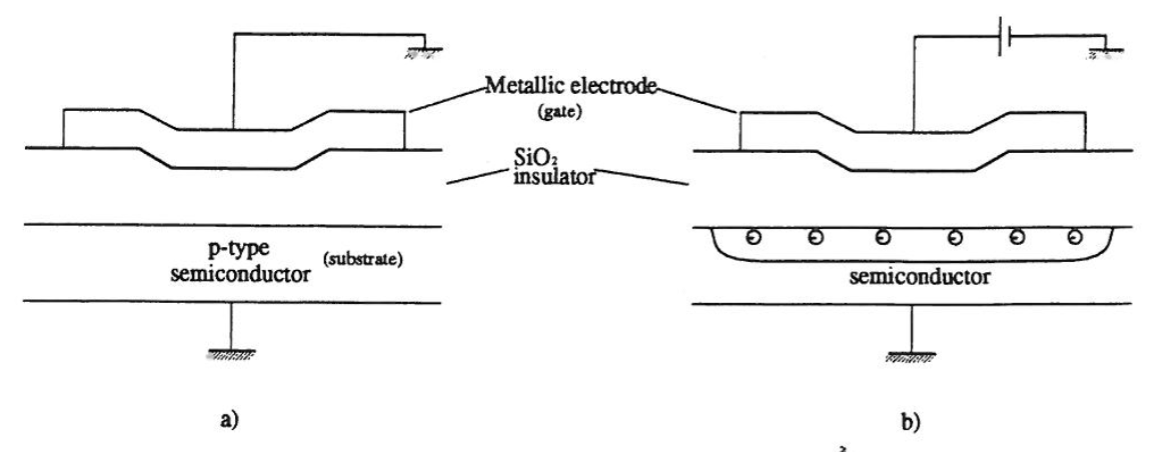
\includegraphics[width=\linewidth]{images/mos}
		\caption{(a) basic MOS capacitor. (b) Depletion Layer under reverse bias \citep[c.f.][fig. 6.20]{hoymorksensors} }
		 \label{fig:mos}
\end{figure}

%If the gate voltage is high enough, an inversion layer forms between the oxide and the depletion layer, which allows 
Due to the photo-electric effect, incoming photons can now generate electron-hole pairs, where the electron is drawn to the positive charged zone and the hole vice versa to the negative charged zone. Therefore, each photon removes a charge from the MOS capacitor, and using a connected charge amplifier, the remaining charge can be converted to a voltage and read out.

 Still, the problem remaining is how to read out individual pixels or MOS capacitors, when there's a large number of them arranged as an array, since connecting every pixel to its individual output amplifier is not suitable or efficient. To cope with this different techniques are used. \par
 According to Hoymark there are four major architectures used for CCD imaging \citep{hoymorksensors}. However, all of them are relying on the same basic principle of charge coupling, which means that the charges accumulated in each pixel are transferred to a charge amplifier by applying appropriate voltages in a time synchronized manner to move charged within the whole CCD device.
 
 The most common techniques are linear shift registers, full frame, frame transfer and the so-called interline transfer.
 For the linear shift register, the simplest of the aforementioned techniques, the CCD is read out horizontally line by line, while the imager or shutter is moving vertically and "scanning" the scene as such.
 The full frame technique uses a global shutter, means the whole CCD is illuminated and read out completely after an appropriate integration time. 
 The third technique, frame transfer is usually used when high frame rates are demanded. Here, only half of the CCD array is illuminated for a specific integration/exposure time and after transferred to the other half where the charges are read out, while the next frame is already captured by the illuminated half.
 However, a disadvantage of the frame transfer technique is "smearing", which means that parts of the captured image are blurry due to the nature of the frame capture.
 Using the interline transfer technique gets rid of this problem by using the CCD 2D array as array of 1D CCD Line sensors. These lines are then connected to an output register which are filled after the line sensors have been illuminated. After, these output register are read out while the next image is already integrated \citep{hoymorksensors}.
 
 Furthermore, the charge coupling can be done using different approaches, more specifically two- three- or four phase cycles which affects the clocking complexity as well as the total amount of gates needed amongst other things \citep{ccdimaging}.
 



%%%%%%%%%%%%%%%%% TASK 2 %%%
\section{CCD Parameters}

\subsection{Spectral radiant incidence}
The spectral radiant incidence, also called irradiance, is the radiant power incident per unit area onto a target and is denoted as \textit{E}. The unit area in this case is the CCD area.
Assuming only small incidence angles and according to Brändström \citep{brandstrom2003auroral} the spectral radiant incidence $E_{\gamma_i}$ is given by:
\begin{equation}
\centering
	\label{eq:irradiance}
	E_{\gamma_i} = T \frac{10^{10}I}{16 {f_{\#}^{2}}} 		
	\hspace{10mm} \si{[{photons} \per\second\meter\squared]}
\end{equation}
where $I$ defines the column emission line, $T$ the transmittance and  $f_{\#}$ the ratio between focal length and aperture stop \citep{brandstrom2003auroral}.



\subsection{Number of incident photons}
The number of incident photons is the number of photons hitting the image plane and can be denoted as
\begin{equation}
\centering
	\label{eq:irradiance}
	n_{\gamma_i} = E_{\gamma_i} t_{int} A_i
	\hspace{10mm} \si{[{photons}]}
\end{equation}

where $t_{int}$ represents the integration time in seconds.
For a CCD sensor with area $A_{CCD}$ the equation is respectively

\begin{equation}
\centering
	\label{eq:irradiance}
	n_{\gamma_{CCD}} = n_{\gamma_i} T_w T_{CCD} \frac{A_{CCD}}{A_i}
	\hspace{10mm} \si{[{photons}]}
\end{equation}

with $T_w$ the transmittance of the CCD-protecting window and $T_{CCD}$ the transmittance of the CCD substrate.

The number of incident photons can also be calculated for one single pixel of the CCD \citep{brandstrom2003auroral}.


\subsection{Quantum efficiency}
Quantum Efficiency (QE) describes the ratio between the photons hitting the CCD and the photons that are actually detected or collected \citep{hoymorksensors}. The Quantum Efficiency can vary throughout the band-pass\footnote{total spectral range for which a detector is sensitive}, thus having different efficiencies for different colors. Modern CCD's have a band-pass of about 3000 to 10000 Å\footnote{1 {Ångström} equals $10^{-10}$ m} and can reach a QE of up to 90\%, while having a QE of 60\% and more for over two thirds of the spectrum \citep{howellCCD}.

%https://www.noao.edu/meetings/gdw/files/Howell_CCDs.pdf

\subsection{Pixel}
A pixel in a CCD device refers to one single unit of a MOS capacitor device, that is able to convert incoming photons to a respective charge, which then can be converted to an appropriate "brightness level" using an charge amplifier and an appropriate ADC as well as specialised software.

\subsection{Noise and its sources}
\label{chap:noise}
According to Hoymork there are three noise sources that have to be considered: read noise, signal shot noise and pixel-to-pixel pattern noise, or, speaking in astronomy terms "read noise limited", "photon noise limited", and "flat field uncertainties" \citep{howellCCD,hoymorksensors}.
At high signal levels the most noise occurs due to pixel-to-pixel sensitivity, which corresponds to the fixed pattern noise in figure \ref{fig:noise}, whereas during low signal levels the limiting noise is the so-called read noise floor, a noise present because of the device properties \citep{hoymorksensors}.

\begin{figure}[!htbp]
	\centering
	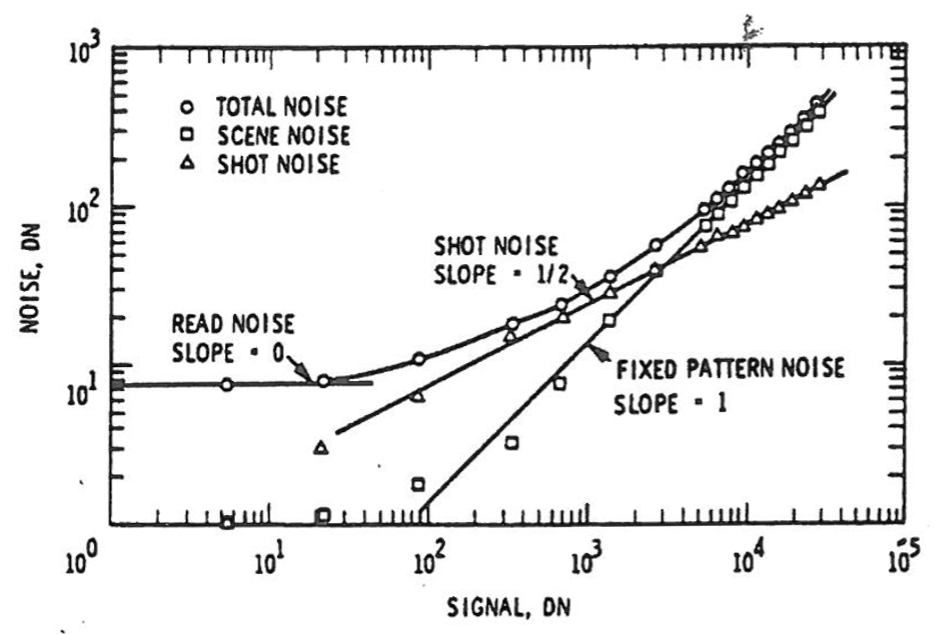
\includegraphics[width=0.8\linewidth]{images/noise}
		\caption{Noise plotted as function of an 20x20 input array \citep[c.f.][fig. 6.24]{hoymorksensors} }
		 \label{fig:noise}
\end{figure}

\subsection{Signal-to-noise ratio for CCD and image intensifier (ICCD)}
In general, the signal-to-noise ratio, in short SNR, characterizes the quality of a measurement. In the case of a CCD the SNR describes the ratio of the total received signal and the combined noise, consisting of the components addressed in chap. \ref{chap:noise} \citep{noiseFSU}. \par
An Intensified CCD (ICCD), is a CCD with an intensifier image tube put in front of the CCD to enhance the sensitivity of the CCD sensor. Applying an intensifier tube reduces the Quantum Efficiency drastically though, which must be considered during design of an instrument or application \citep{hoymorksensors}.

\subsection{Noise- and Saturation Equivalent Exposure}
The Noise Equivalent Exposure is defined as a SNR of 1, which means that signal after exposing/integrating has the same strength as the combined system noise, rendering the measurement more or less unusable. According to Brändström the Detection Threshold is located at an SNR of around 2 \citep[c.f.][chap. 3.1.10]{brandstrom2003auroral}.

The Saturation Equivalent Exposure is the exposure/integration after which the well capacity of the single MOS capacitors of the CCD is fully exhausted. This leads to saturation, as the name implies. Further illumination or more exposure can not be detected \citep{brandstrom2003auroral}.

\subsection{Dynamic Range}
The Dynamic Range (DR) of a sensor is given in dB and is the peak signal divided by the Root-Mean-Square noise and the DC bias level.

In other words, it is the peak signal, which means the maximum achievable signal defined by the well capacity, divided by the sum of noises of the system. For practical applications this means that the higher the dynamic range is, the better low intensity signals are being detected.


\begin{figure}[!htbp]
	\centering
	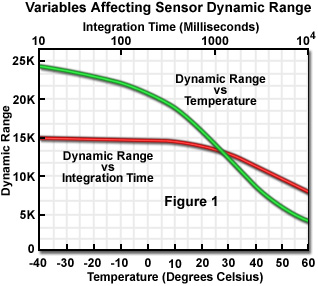
\includegraphics[width=0.6\linewidth]{images/dynrange}
		\caption{Dynamic Range and its Variables \citep[c.f.][\href{https://micro.magnet.fsu.edu/primer/digitalimaging/concepts/images/dynamicrangefigure1.jpg}{Dynamic Range Figure}]{ccdimaging} }
		 \label{fig:dynrange}
\end{figure}







%%%%%%%%%%%%%%%%% TASK 3 %%%
\section{CCD Elements for ALIS}
ALIS is an Auroral Large Imaging System proposed by Åke Steen in 1989 to automate auroral imaging stations in Scandinavia. The following chapters describe different elements of the CCD chosen for this specific project \citep{brandstrom2003auroral}.

\subsection{Optical system}
The optical system of ALIS had different very specific constraints in the beginning of the project, as replaceable front lenses, a filter wheel in front of the lenses and a changeable field of view. These specifications were cut down due to budget issues and the final set up of the optical system is given in the picture below.

\begin{figure}[!htbp]
	\centering
	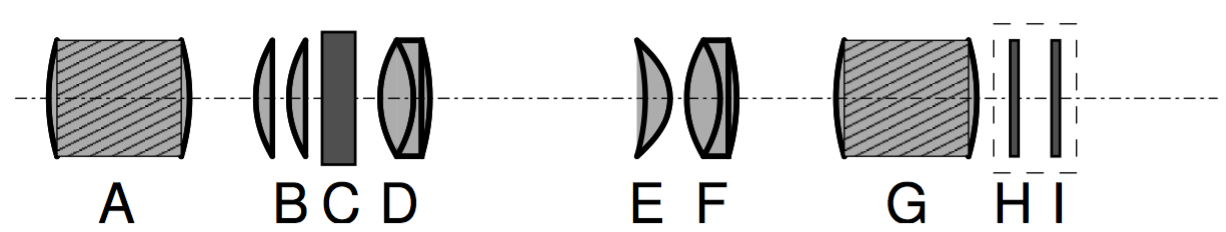
\includegraphics[width=0.8\linewidth]{images/optsys}
		\caption{(A) replacable front lens, (B) telecentric lenses to have parallel light rays coming in, (C) filter holder, (D) field-lens, (E) \& (F) close up lenses, (G) Camera lens, (H) Window of CCD enclosure, (I) CCD sensor \citep[c.f.][Fig. 3.7, modified]{brandstrom2003auroral}}
		 \label{fig:optsys}
\end{figure}

\subsection{Interference filters}
\label{interference}
The interference filters mounted in the filter holder (c.f. Fig. \ref{fig:optsys}.(C)) used in ALIS are so-called Fabry-Perot filters. They are narrow-band filters to enable spectroscopic imaging of different wavelength. Since these filters require the incoming light to be almost perfectly normal to the filter plane, the aforementioned tele-centric must be used.
Due to this fact in ALIS the filters are desired to be insensitive against the angle of incoming rays, as well as having a wide enough bandwidth to pass the desired wavelength at all angles, which is why the filters are usually custom made for a specific application, and therefore are quite expensive. \par
In case of ALIS, the filter wheel contains six different filters in the filter wheel, namely 5577Å (O($^1$S)), 6300Å (O($^1$D)), 6230Å, 5324Å, 4278Å and an empty filter box for white light. Using the appropriate filter, different areas of application are covered, e.g. meteor studies, background light filters, LIDAR and auroral emission (mainly using the N$^2_+$ 1Neg. filter)\citep{brandstrom2003auroral}.

\subsection{Camera positioning system}
Since ALIS uses a non-changeable FOV, the imager must be moved to comply with different imaging modes, as there are the tomographic mode, maximum sky coverage mode or spacecraft foot-point tracking. This is why not a simple azimuth/elevation system is used, but a frame-based system was developed, using three frames mounted in each other, where the imager is mounted on the innermost frames, while the two innermost frames are mounted on perpendicular axes. The frames itself are moved with the help of stepper motors.

Using this system one can avoid the cable wrapping problem and keep the cables nice and short, but still reach all regions in the sky.



%%%%%%%%%%%%%%%%% TASK 4 %%%
\section{Scientific results of ALIS}
Due to the complex nature of the Auroral Large Imaging System project, there were various different scientific objectives pursued, of which some are now looked deeper into.

\subsection{Estimation of auroral electron spectra}
The conventional choice of emission lines for monochromatic auroral imaging used to be 6300Å (O($^1$D)) emission line, as mentioned in chapter \ref{interference}. But since this emission line has a long radiative lifetime and is not available in lower altitudes, the N$_2^+$ 1Neg. 4278Å line is used as well for the characteristic energy of incoming electrons \citep{brandstrom2003auroral}.

At March 25th, 1998 it was also discovered, that the emission line of O(3p$^3$P) at 8446Å, especially the morphology of the aurora is similar to that of N$_2^+$ 1Neg. 4278Å \citep{brandstrom2003auroral}.
Newer and more extensive studies, performed by Gustavsson et al. in 2001 \citep{brandstrom2003auroral}, have shown that with the inverse of the N$_2^+$ 1Neg. 4278Å altitude distribution the characteristics of primary electron spectra can be estimated with a time resolution of about 10s for discrete auroral structures. 
To retrieve useful results for variations slower than 100s the measurements of 4278Å, 6300Å and 8446Å emission lines can be combined, but according to Gustavsson 2D measurements are needed to distinguish between spatial and temporal variations, especially for these kinds of events \citep{brandstrom2003auroral}.


\subsection{Auroral vorticity}
The auroral arc that extends from east to west is often destroyed by instability processes, that also create vortex-like structures, whereas the vorticity $\zeta$ is defined as the rotation in a fluid, denoted by $\zeta = \nabla \times \textbf{u}$ \citep{brandstrom2003auroral,pudovkin1997vorticity}.
\begin{figure}[!htbp]
\captionsetup{width=0.6\textwidth}
	\centering
	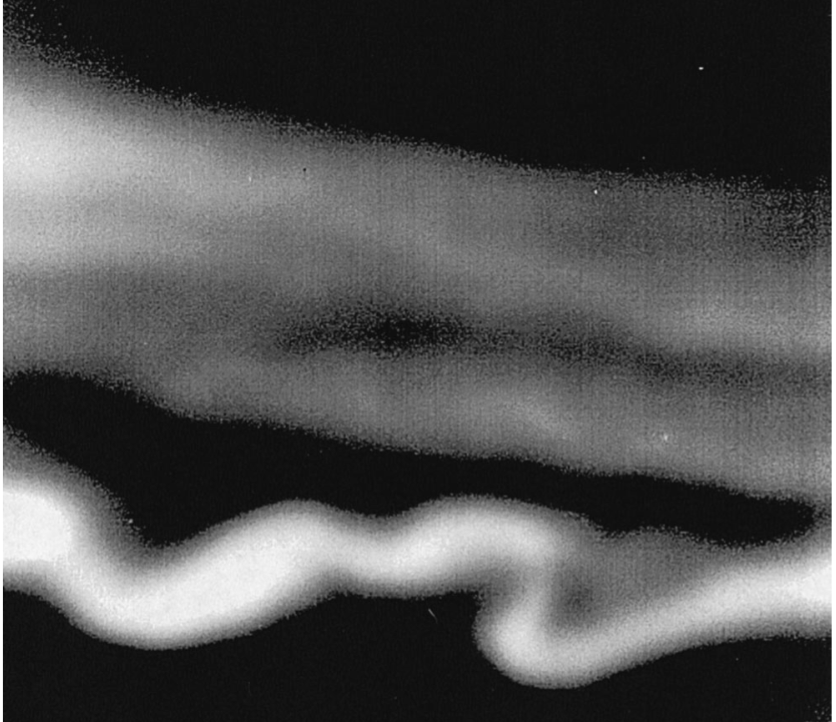
\includegraphics[width=0.6\linewidth]{images/vortex}
		\caption{ALIS data showing a vortex formation, gathered at the Kiruna station at 5577Å (\citep[c.f.][Fig. 14a, modified]{pudovkin1997vorticity})}
		 \label{fig:vortex}
\end{figure}
Using early ALIS image data as in Fig. \ref{fig:vortex} Pudovkin was able to study the vorticity in magnetospheric plasma and its effects on auroras.
Amongst other things, these studies were done to determine distributions of electric fields and currents in the magnetosphere as well as observing MHD\footnote{Magnetohydrodynamical} instabilities, which are basically responsible for the turbulences. Unfortunately, due to the insufficient temporal resolution the ALIS project was not perfectly suited for this kind of research \citep{brandstrom2003auroral}.

\subsection{Ionospheric trough}
An ionospheric trough is a region in the F layer where the plasma density is significantly decreased \citep{spacewiki}. This trough is usually observed with the more direct measurement methods of the EISCAT radar, but it was occasionally detected that ALIS is able to provide supporting measurements, which correlate very well with extrapolated EISCAT measurements concerning the position of diffuse aurora in the ionospheric trough. The result of these observations was the discovery that early proposals for the linear equations of trough motion were not valid in the observed latitude range \citep{brandstrom2003auroral}.

\subsection{Daytime auroral imaging}
Usually the ALIS system is shut down during the arctic day season, from 15th April to August/September, since the nights are too bright at these latitudes for ALIS performing its measurements. Nevertheless, a prototype imaging spectrometer has been built to enable ALIS for daylight aurora imaging \citep{brandstrom2003auroral}.

This prototype used capacitance-stabilised Fabry-Perot etalons as well as narrow-band interference filters of 2Å. By fine-tuning the spectrometer with the etalons to 6300Å, it was possible to reconstruct a 2D sky image. Still, the emission line was only roughly estimated, since the solar spectrum had to be substracted from the measurements and a previously published spectrum was used to perform the subtraction instead of using a specific measurement of the solar spectrum. Still, with slight modifications this instrument could be used for daylight aurora imaging, but with only low temporal resolution \citep{brandstrom2003auroral}.

\subsection{Auroral events and thermospheric neutral wind}
The Magnetosphere and the thermo- and ionosphere are coupled by electric fields and field-aligned currents.
Combining the ALIS high-res aurora images with the neutral wind vector measurements of the Fabry-Perot interferometer leads to a better understanding the mentioned coupling.\\
Experiments and measurements have been carried out since the 1980s and provided some interesting results. It was discovered that the neutral wind was oriented mostly northward when a stable aurora arc was seen. An in-depth analysis revealed that the wind is directed perpendicular to the arc, with low wind speed in parallel. Also, diffuse auroral structures seem to drift westward, when the wind turns in eastern direction, at around 19:30 UTC \citep{brandstrom2003auroral}.

\subsection{Meteor studies}
Another interesting aspect of the ALIS project is the ability to observe different ablation phenomena in meteoroid trails passing the earth, where the easiest observable meteoroid constituents are Natrium and Calcium, since they have very strong emission lines at 5893Å and 4227Å. To observe these fast occurring events the ALIS imagers worked in a matter, so that always at least two imagers had open shutters, to overlap exposures and capture meteoroid trails.
Different studies have been performed, especially on the Leonid showers, whereas not all studies have been successful due to cloudy weather conditions.\\
One of the more surprising results was the detection of a fast fainting emission line in 4227Å at a height of 160km and 130km. These emission lines were explained only long after the initial measurement, stating that the water bound to the meteoroid is heated up very fast and released suddenly in a bright process, resulting in very bright meteoroid trails.

%%%%%%%%%%%%%%%%% TASK 4 %%%
\section{CCD comparison of ALIS and onboard Earth auroral imaging}
Compared to the ALIS Index Camera
The MAC\footnote{Multi-spectral auroral camera} of the REMEI and the INDEX satellite are, due to the nature of the working environment very different from the one used at ALIS.
The first that one may notice is the different construction. The on-board cameras have no movable parts like the movable filter and changeable lenses at ALIS, but they have three CCD sensors with each attached to an lens and interference filter. Obviously, the advantage of this setup is the ability to observe an event in three different wavelength's simultaneously. Also, the device is mounted on the satellite's structure, not as the ALIS device within a movable set of frames. The disadvantage of this setup is that the whole satellite has to be moved, if another region has to be observed, although won't be very large, since the satellites are observing the earth from an orbit at around 600km. Also, the calibration of the setup is harder to perform for the on-board MAC, since there is no possibility to fine-tune the instruments in orbit, as there is for the ALIS setup. \citep{sakanoi2003development,obuchi2008initial,brandstrom2003auroral}.

The three different wavelength that can be observed with the two on-board cameras are 4278Å (N$_2^+$1N), 5577Å (OI) and 6700Å (N$_2$1P), which is similar to the ones used in ALIS. The advantage of ALIS is in this case that, with movable filters the number of observable emission lines can be much higher, whereas the filters used in the satellite have to be as small and as light as possible, to reduce launch costs \citep{obuchi2008initial}.
The filters used in the INDEX satellite differ very slightly from the ones used in REIMEI, namely 4282Å, 5580Å and 6717Å \citep{sakanoi2003development}.

Furthermore, another important aspect are the different FOVs. Both satellites use an FOV of 7.6°, while the ALIS system uses 50° for more coverage. This small FOV enables the satellites to observe even very fine auroras, with an total footprint area of 70km square, if assumed that auroras are at about 110km above ground \citep{obuchi2008initial}.
Also, the Quantum Efficiency of the sensors used differ, while the sensor size is equal for all sensors with 1024x1024 pixels. The onboard satellites have a QE of about 0.6, while the ALIS CCD goes up to 0.9, obviously depending on the respective emission lines observed \citep{obuchi2008initial,brandstrom2003auroral}.

In general using image sensors in space poses more risks and technical challenges than using them on earth, since one has to take care not only about the overall structure but also for appropriate power supplies and thermal control, because the noise in captured images increases with temperature, as has been explained during the first chapters of this report. Still, the big advantage is the possibility of large scale observations of large events on earth or in the earth atmosphere, as would not be possible from earth.

%%%%%%%%%%%%%%%%% TASK 5 BONUS %%%
\section{Literature Survey}
Since the available literature on thermospheric neutral wind and meteor studies with the ALIS system and its scientific results date back to 2003, a short survey on further recent research is given.

The particular field of thermospheric neutral winds got a lot of attention in recent years and amongst others NASA and JAXA/SAS were launching sounding rockets to study the neutral wind, since it is a key parameter for the ionosphere thermosphere coupling. Watanabe et al. focused their research in their Paper \textit{Neutral Wind Observations below 200 km altitudes (2015)} especially on neutral winds below 200km and had some interesting findings especially concerning Lithium clouds. It was also the first time that a technique called moon light scattering was used for thermospheric wind measurement in midnight.

Also, Swenson et al. recently used LIDAR to measure and map thermospheric the first time in lower thermosphere (at around 130km). In their paper \textit{Na Lidar measurement of neutral wind and temperature in the lower thermosphere (2015)} they also propose future LIDAR measurement of thermospheric neutral properties.

Concerning meteoroid studies using imaging techniques, these techniques are more and more used to study the composition of meteoroids, as is described by Jenniskens et al. in their publication \textit{Spectroscopic anatomy of a meteor trail cross section with the European Southern Observatory Very Large Telescope}.\\
Also, a team led my Madiedo in the S.M.A.R.T. Project uses different spectrographs all around spain to perform a systematic analysis of incoming meteors and meteoroids. This project automatically scans and saves information about meteors entering or passing the earth and dissects its composition fully autonomous, as is described in the publication \textit{Recent developments in meteor spectroscopy in the framework of the S.M.A.R.T. project (2014)}.

Although, Meteoroid studies are not only done on earth, but also e.g. on Mars, where MAVEN, a imaging UV spectrograph is used to detect meteoroid showers.

The trend of these spectrographic methods goes into the direction of more and more automation, especially since sophisticated algorithms are developed and computer performance is constantly increasing. Roman and Buiu for example developed an artificial neural network (ANN) which is developing its own ability to detect meteoroids the more meteoroid it detects. The results of this approach were published in \textit{Automatic detection of meteors using artificial neural networks (2014)}.


